\documentclass[12pt]{article}
\usepackage[margin=2.5cm]{geometry}
\usepackage{enumerate}
\usepackage{amsfonts}
\usepackage{amsmath}
\usepackage{fancyhdr}
\usepackage{amsmath}
\usepackage{amssymb}
\usepackage{amsthm}
\usepackage{mdframed}
\usepackage{graphicx}
\usepackage{subcaption}
\usepackage{adjustbox}
\usepackage{listings}
\usepackage{xcolor}
\usepackage{courier}
\usepackage[utf]{kotex}
\usepackage{hyperref}
\usepackage{soul}

\definecolor{codegreen}{rgb}{0,0.6,0}
\definecolor{codegray}{rgb}{0.5,0.5,0.5}
\definecolor{codepurple}{rgb}{0.58,0,0.82}
\definecolor{backcolour}{rgb}{0.95,0.95,0.92}

\lstdefinestyle{mystyle}{
    backgroundcolor=\color{backcolour},
    commentstyle=\color{codegreen},
    keywordstyle=\color{magenta},
    numberstyle=\tiny\color{codegray},
    stringstyle=\color{codepurple},
    basicstyle=\ttfamily\footnotesize,
    breakatwhitespace=false,
    breaklines=true,
    captionpos=b,
    keepspaces=true,
    numbers=left,
    numbersep=5pt,
    showspaces=false,
    showstringspaces=false,
    showtabs=false,
    tabsize=1
}

\lstset{style=mystyle}

\pagestyle{fancy}
\renewcommand{\headrulewidth}{0.4pt}
\lhead{CSC 369}
\rhead{Midterm 4 Solution}

\begin{document}
\title{CSC 369 Midterm 4 Solution}

\bigskip

\begin{enumerate}[1.]
    \item

    \begin{enumerate}[a)]

        \item
        \begin{enumerate}[1)]
            \item 4 - inode blocks. 1 for the file \texttt{c}, and 3 for the
            directdories \texttt{/}, \texttt{a}, \texttt{b}

            \item 3 - directory blocks - one for root \texttt{/}, one for \texttt{a},
            the other for \texttt{b}

            \item 1 - single indirect block as far as we know. The file definitely has more than
            12 blocks (\# of data blocks pointed by direct pounters), but less than 1036 (\# of data blocks pointed
            by direct pointers and single indirect pointers). We are reading block 1034.

            \item 1 - data block for file \texttt{c}
        \end{enumerate}

        \item

        All of the above

        \bigskip

        \underline{\textbf{Notes}}

        \begin{itemize}
            \item \textbf{Inode}

            \begin{center}
            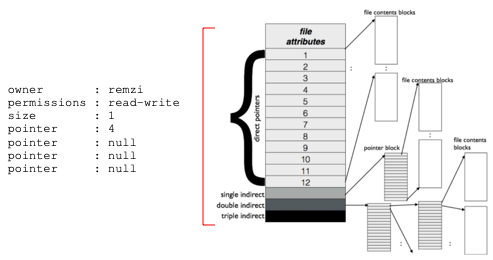
\includegraphics[width=0.6\linewidth]{../images/midterm_4_solution_1.png}
            \end{center}

            \begin{itemize}
                \item Is short form of \textbf{index node}
                \item Describes a file system object such as file or data
                \item Contains all information about a file/directory, including
                \begin{itemize}
                    \item File Type,
                    \item Size
                    \item Number of blocks allocated to it
                    \item Protection information
                    \item Time information (e.g time created, time modified)
                    \item Location of data blocks residing on disk
                \end{itemize}

            \end{itemize}
        \end{itemize}

        \bigskip

        \underline{\textbf{References}}

        \begin{enumerate}[1)]
            \item Wikipedia, Inode, \href{https://en.wikipedia.org/wiki/Inode}{link}
            \item Machanick, Philip. (2016). Teaching Operating Systems: Just Enough Abstraction. 642. 10.1007/978-3-319-47680-3\_10., \href{https://www.researchgate.net/figure/Conceptual-index-node-inode-The-top-level-block-contains-file-attributes-12-direct_fig1_306347325}{link}
        \end{enumerate}

        \item

        Size, the location of data blocks that reside on disk

        \bigskip

        \underline{\textbf{Notes}}

        \begin{itemize}
            \item I wonder what information about blocks inode has. Is it total number
            of blocks both inode and data, or just data?
            \item I struggled a bit on this one. I should find an easier way to
            remember which information inode has
        \end{itemize}

        \item

        \bigskip

        \underline{\textbf{Rough Work}}

        \begin{itemize}
            \item \textbf{Creash Scenarios}

            \begin{itemize}
                \item When only new data block is written to disk

                \begin{itemize}
                    \item This is fine in system's point of view
                    \item No inode points to it (it doesn't contain any information about file)
                    \item No bitmap points to it
                    \item Is as if write never occured
                \end{itemize}
                \item When only the updated inode is written to disk
                \begin{itemize}
                    \item There is no bitmap that's pointing to it
                    \item There is new inode where existing inode is
                    \item The data block \texttt{Db} hasn't been created
                    \item Reading data where \texttt{Db} is will return garbage data
                    \item there is a term for this. Is called \textbf{File-System inconsistency}
                \end{itemize}
                \item When only inode bitmap is written to disk

                \begin{itemize}
                    \item inode block pointed by bitmap is assumed to be allocated
                    \item But there is no desired inode where it's pointing
                    \item This is another example of \textbf{File-System-Inconsistency}
                    \item If left as is, then space cannot be used for future use (\textbf{inode leak})
                \end{itemize}
                \item When only data bitmap is written to disk

                \begin{itemize}
                    \item data block pointed by bitmap is assumed to be allocated
                    \item But there is no desired inode where it's pointing
                    \item This is another example of \textbf{File-System-Inconsistency}
                    \item If left as is, then space cannot be used for future use (\textbf{data leak})
                \end{itemize}
            \end{itemize}
        \end{itemize}

        \bigskip

        \underline{\textbf{Notes}}

        \begin{itemize}
            \item I wonder how system call for reading file/directory works in UNIX. Does it check for bitmap?
            \item I wonder how system call for deleting file/directory works in UNIX
            \item I wonder how system call for creatubg file/directory works in UNIX

            \item \textbf{File API}
            \begin{itemize}
                \item \texttt{open} (create)
                \begin{itemize}
                    \item Is a system call
                    \item \textbf{Syntax:}

                    \bigskip

                    \texttt{int fd = open("foo". O\_CREAT|O\_WRONLY|O\_TRUNC, S\_IRUSR|S\_IWUSR)}

                    \bigskip

                    \begin{itemize}
                        \item \texttt{O\_CREAT} - Creates file "foo" if does not exist
                        \item \texttt{O\_WRONLY} - Open file for writing only (default)
                        \item \texttt{O\_TRUNC} - Overwrites existing file \color{red}Need example/Clarification\color{black}
                        \item Can have multiple flags
                    \end{itemize}
                    \item Returns \textbf{file descriptor} or \texttt{fd} for short

                    \begin{itemize}
                        \item Is an integer
                        \item Is used to access a file
                        \item Is \underline{private} per process
                        \item Can be used to \texttt{read()} and \texttt{write()} files
                    \end{itemize}

                    \bigskip

                    \underline{\textbf{Example}}

                    \bigskip

                    \begin{center}
                    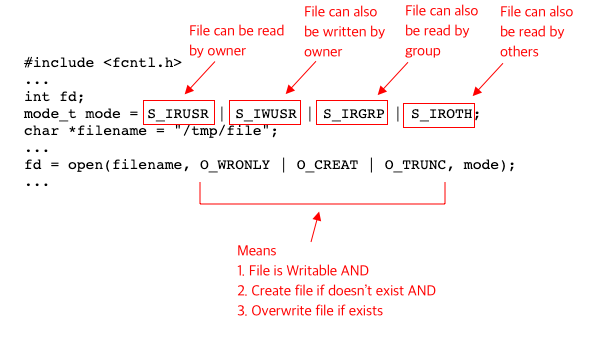
\includegraphics[width=\linewidth]{../images/midterm_4_solution_2.png}
                    \end{center}
                \end{itemize}

                \item \texttt(read)
                \begin{itemize}
                    \item Is a system call
                    \item \textbf{Syntax:}

                    \bigskip

                    \texttt{ssize\_t read (int fd, void *buf, size\_t count)}

                    \bigskip

                    \begin{itemize}
                        \item \texttt{fd} - file descriptor (from \texttt{open()})
                        \item \texttt{buf} - container for the read data
                        \item \texttt{count} - number of bytes to read
                    \end{itemize}
                    \item Returns number of bytes read, if successful
                    \item Returns 0 if is at, or past the end of file

                    \bigskip

                    \underline{\textbf{Example}}

                    \bigskip

                    \begin{center}
                    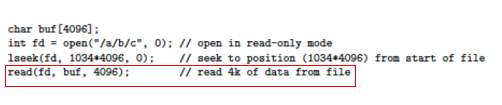
\includegraphics[width=\linewidth]{../images/midterm_4_solution_3.png}
                    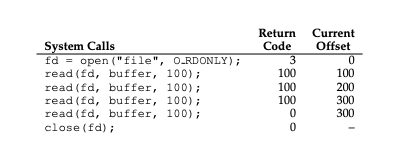
\includegraphics[width=\linewidth]{../images/midterm_4_solution_5.png}
                    \end{center}

                \end{itemize}

                \item \texttt{write}

                \begin{itemize}
                    \item Is a system call
                    \item Writes data out of a buffer
                    \item \textbf{Syntax:}

                    \bigskip

                    \texttt{ssize\_t write (int fd, const void * buf, size\_t nbytes)}

                    \bigskip

                    \begin{itemize}
                        \item \texttt{fd} - file descriptor
                        \item \texttt{buf} - A pointer to a buffer to write to file
                        \item \texttt{nbytes} - number of bytes to write. If smaller than buffer, the output is truncated
                    \end{itemize}
                \end{itemize}

                \bigskip

                \underline{\textbf{Example}}

                \bigskip

                \begin{center}
                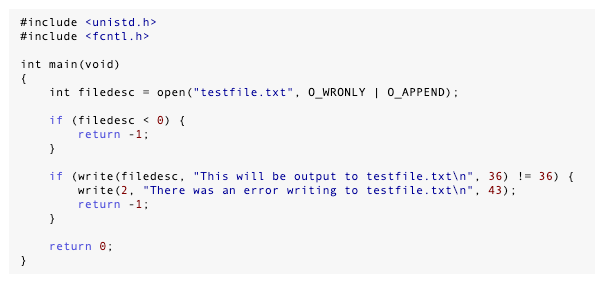
\includegraphics[width=\linewidth]{../images/midterm_4_solution_4.png}
                \end{center}

                \item \texttt{lseek}

                \begin{itemize}
                    \item Reads or write to a specific offset within a file
                    \item \textbf{Syntax:}

                    \bigskip

                    \texttt{off\_t lseek (int fd, off\_t offset, int whence)}

                    \bigskip

                    \begin{itemize}
                        \item \texttt{fd} - file descriptor
                        \item \texttt{offset} - the offset of pointer within file (in bytes)
                        \item \texttt{whence} - the method of offset

                        \bigskip

                        \quad \texttt{SEEK\_SET}  - offset from the start of file (absolute)

                        \quad \texttt{SEEK\_CUR} - offset from current location + offset bytes (relative)

                        \quad \texttt{SEEK\_END} - offset from the end of file
                    \end{itemize}

                    \item Returns offset amount (in bytes) from the \underline{beginning} of file
                    \item Returns -1 if error
                \end{itemize}

                \bigskip

                \underline{\textbf{Example}}

                \begin{center}
                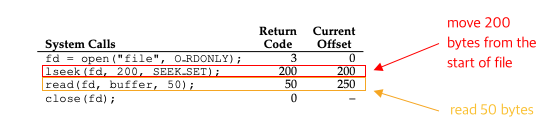
\includegraphics[width=0.8\linewidth]{../images/midterm_4_solution_7.png}
                \end{center}

                \item \texttt{rename}

                \begin{itemize}
                    \item Changes the name of file
                    \item \textbf{Syntax:} \texttt{int rename(const char *old, const char *new)}

                    \begin{itemize}
                        \item
                    \end{itemize}
                \end{itemize}
            \end{itemize}

            \item \textbf{Reading and Writing Files}
            \item \textbf{Reading and Writing Files}
            \item \textbf{Renaming Files}
            \item \textbf{Removing Files}
            \item \textbf{Making Directories}
            \item \textbf{Reading Directories}
            \item \textbf{Removing Directories}
            \item \textbf{Hard Links}
            \item \textbf{Symbolic Links}
        \end{itemize}

    \end{enumerate}
\end{enumerate}


\end{document}